\section{Resultat af tegning}

\begin{figure}[h]
        \centering
        	\begin{subfigure}[b]{0.3\textwidth}
                	\includegraphics[scale=0.040]{Billeder/Bedst-Billede.jpg}
               		\caption[caption]{Robottens tegning af figur~\ref{fig:Bedst-Billede-Original}}
            	    \label{fig:Bedst-Billede}
       		\end{subfigure}
       		\quad%
        ~ %add desired spacing between images, e. g. ~, \quad, \qquad, \hfill etc.
          %(or a blank line to force the subfigure onto a new line)
       		\begin{subfigure}[b]{0.3\textwidth}
                	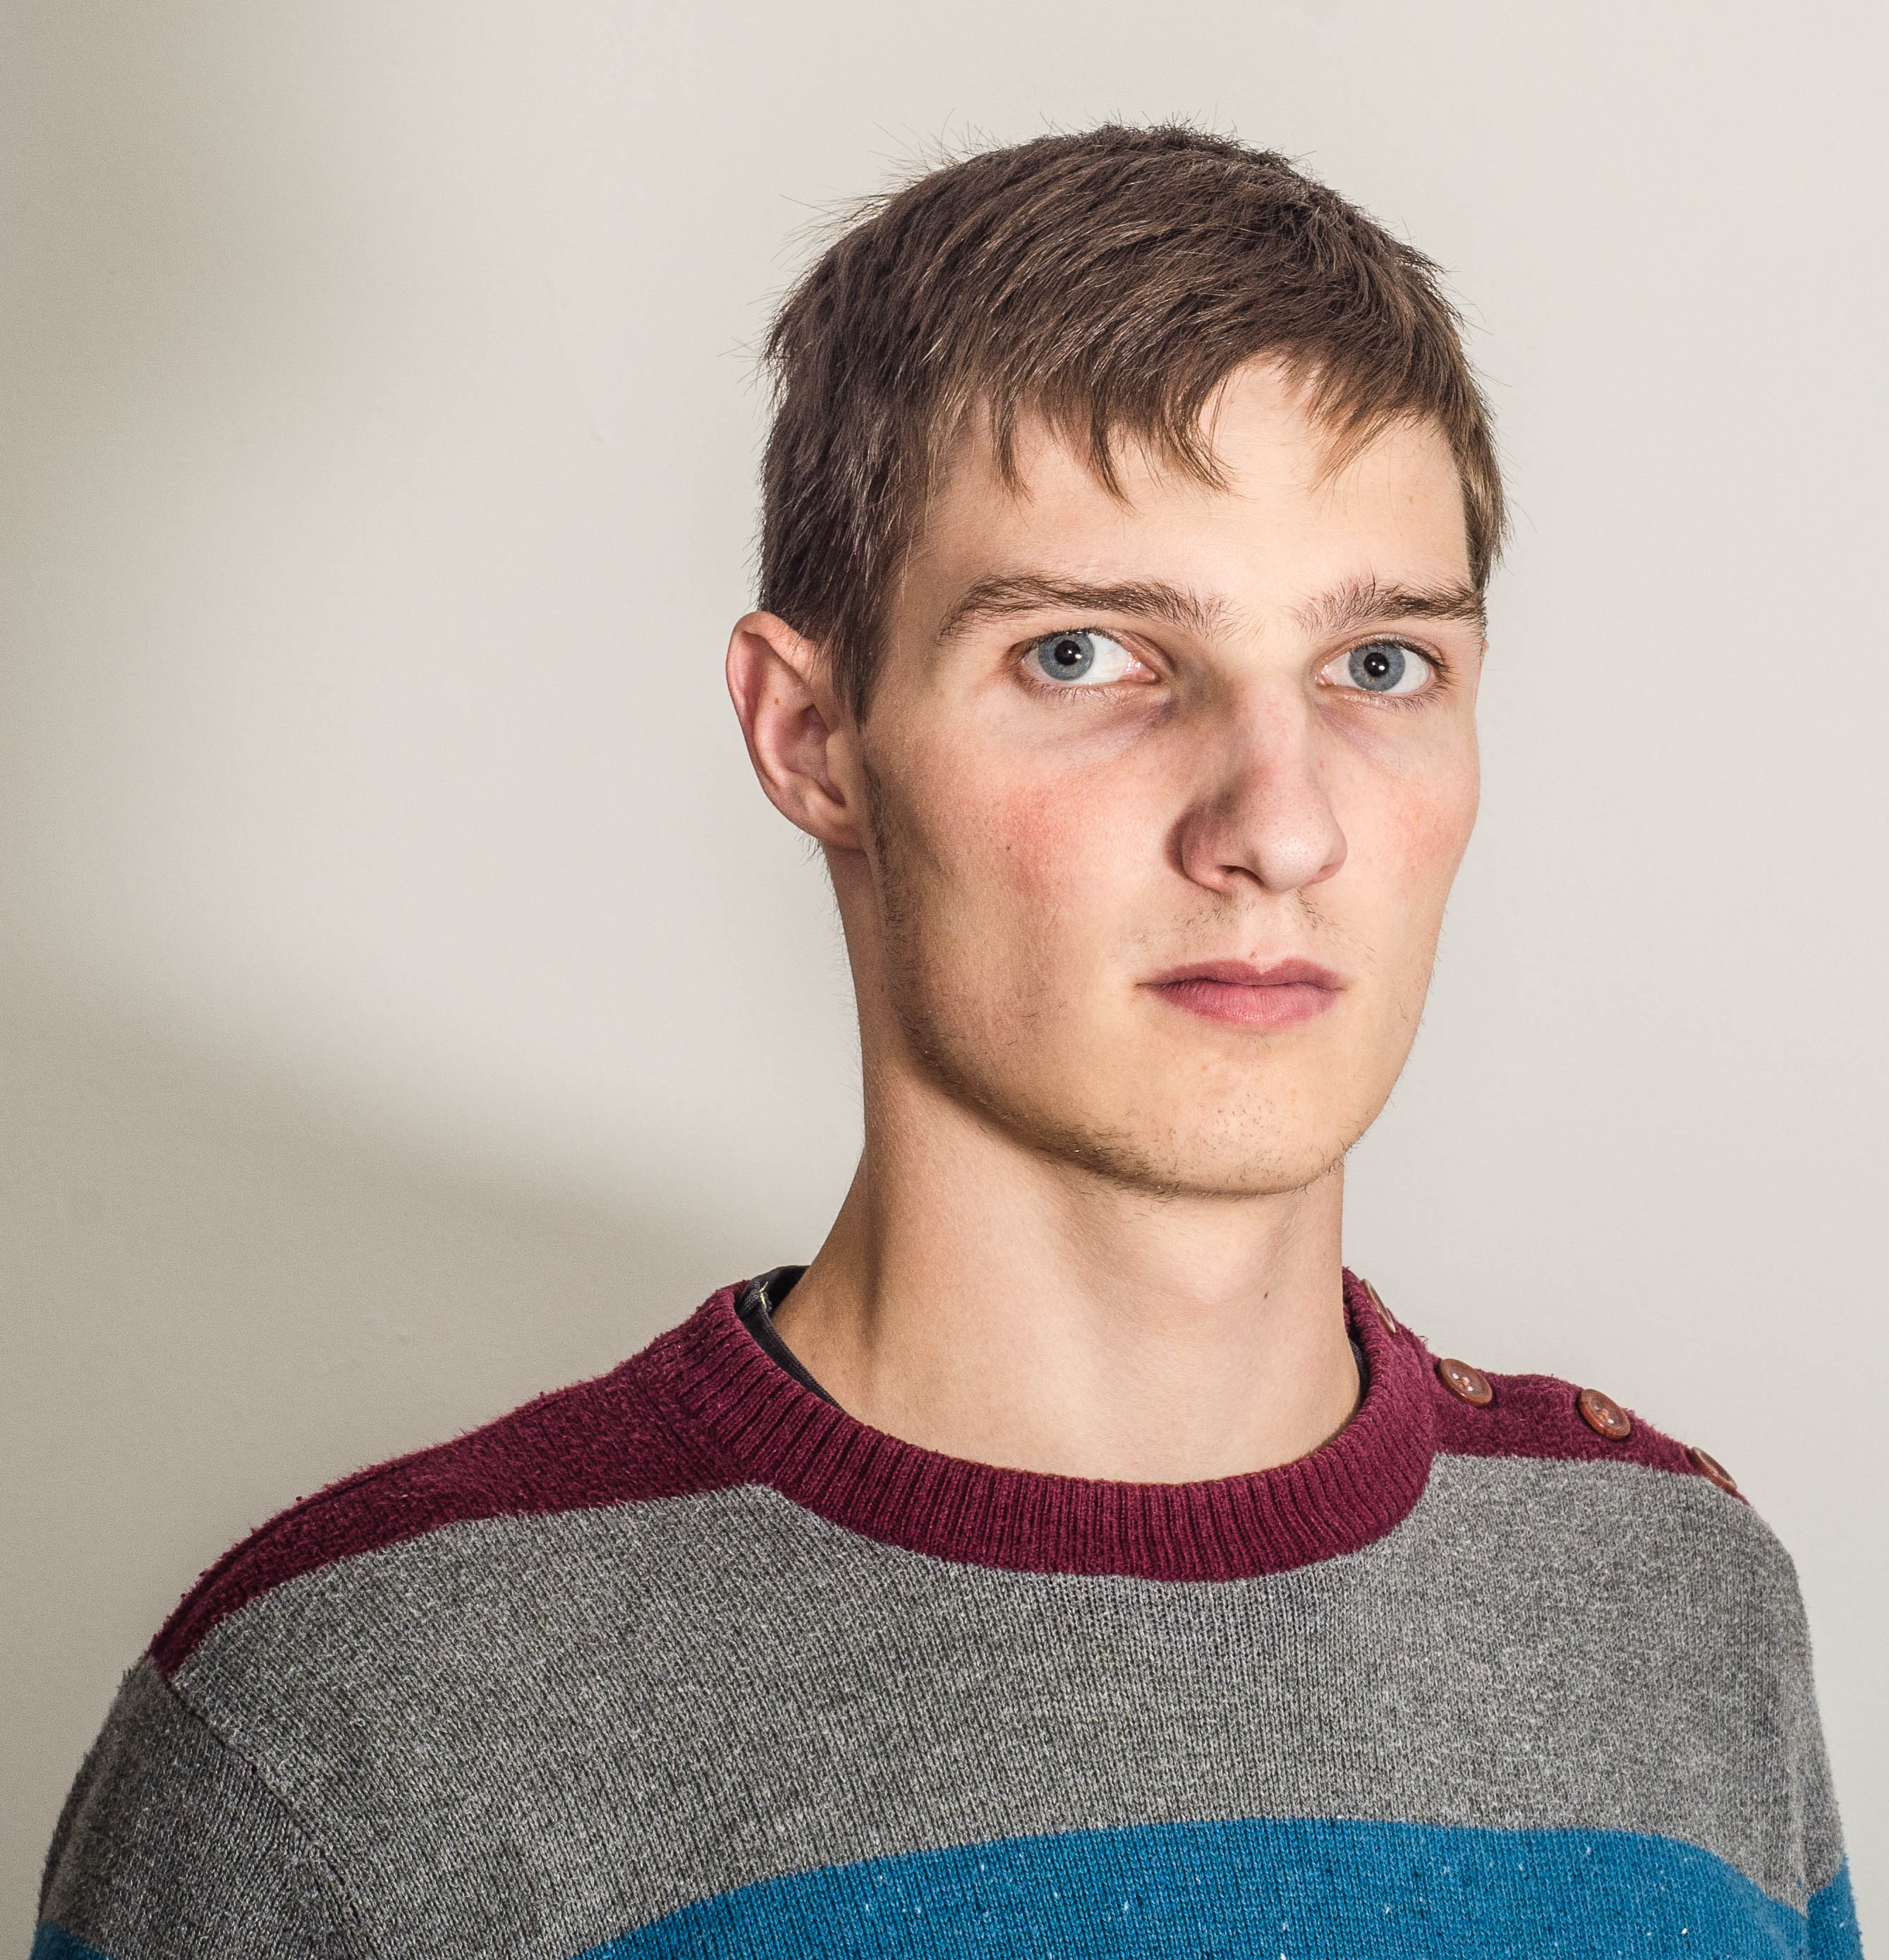
\includegraphics[scale=0.045]{Billeder/Bedst-Billede-Original.jpg}
            	    \caption[caption]{Orignalt billede\\
            		\ }
          	      \label{fig:Bedst-Billede-Original}
        	\end{subfigure}
        	\caption[caption]{Sammenligning af tegning og billede}
        	\label{fig:William-med-tre-farver}
\end{figure}

Som det kan ses på figur~\ref{fig:William-med-tre-farver}, kan man tydeligt se forskel på de tre forskellige farver i billedet. Det giver den ønskede effekt og giver muligheden for at tegne mange forskellige billeder. Så længe billedet ikke er for monotont i farve og belysning, er der stort set mulighed for at tegne alt. Derudover kan det programmerede kode indstilles, til at tegne pæne logoer, hvor der ikke er fokus på farvenuancer, men på hårde og skarpe kanter. På figur~\ref{fig:Segl-SDU} ses et logo tegnet med samme program, hvor logo er valgt som indstilling.

\begin{figure}[h]
        \centering
        	\begin{subfigure}[b]{0.3\textwidth}
                	\includegraphics[scale=0.040]{Billeder/Tegning-SDU-Segl.jpg}
               		\caption[caption]{Robottens tegning af figur~\ref{fig:Bedst-Segl-SDU-Original}}
            	    \label{fig:Bedst-Segl-SDU}
       		\end{subfigure}
       		\quad%
        ~ %add desired spacing between images, e. g. ~, \quad, \qquad, \hfill etc.
          %(or a blank line to force the subfigure onto a new line)
       		\begin{subfigure}[b]{0.3\textwidth}
                	
\includegraphics[scale=0.45]{Billeder/Segl-SDU.jpg}
            	    \caption[caption]{Orignalt billede\\
            		\ }
          	      \label{fig:Bedst-Segl-SDU-Original}
        	\end{subfigure}
        	\caption[caption]{Sammenligning af tegning og billede}
        	\label{fig:Segl-SDU}
\end{figure}


Som det ses på figur~\ref{fig:Segl-SDU}, er det muligt at tegne logoer. Dette er SDU's logo, tegnet hvor kanten er tegnet. Det kunne også laves således, at både kanten og fyldet er lavet. Det ses på figuren som er lavet med 500 pixels, at tegningen er meget eksakt. Denne ville være betydeligt mere upræcis hvis den var lavet med færre pixels.